\documentclass{article}
\usepackage[utf8]{inputenc}
\usepackage{graphicx}

\RequirePackage[T1,TS1,T2A]{fontenc}
\RequirePackage[english,russian]{babel}   %% загружает пакет многоязыковой вёрстки

% Formatting
\RequirePackage[left=2.5cm, right=2cm, top=2cm, bottom=2.5cm]{geometry}

\usepackage{hyperref}
\usepackage[usenames,dvipsnames,svgnames,table,rgb]{xcolor}

\title{Расчет дисперсионной кривой}
\author{Тимур Базаров}
\date{март 2020}

\begin{document}
\maketitle

\textbf{Цель:} рассчитать дисперсионную кривую с учетом реального фотоприемника


\section{Введение}
За основу взята статья Optical receiver performance evaluation.

\section{Формулы для расчета влияния экстинкции}

\begin{equation}
    Q=\frac{V_1-V_0}{\sigma_1+\sigma_0}
\end{equation}

\textbf{Это выражение можно понимать как частное размаха и удвоенного шума}.
%\begin{equation}
    %BER=\frac{1}{2}erfc\left(\frac{Q_{BER}}{\sqrt{2}}\right)
%\end{equation}
Таким образом, шум тока на входе в TIA $N_{TOTAL}$, соответствующий определенному BER можно пересчитать в минимальный размах тока $I_{P-P}$:

\begin{equation}
    I_{P-P}=2\times Q_{BER}\times N_{TOTAL}
\end{equation}

Размах можно пересчитать в среднюю величину, зная экстинкцию:

\begin{equation}
    I_{av}=\frac{I_{P-P}\times(ER+1)}{2\times(ER-1)}=Q_{BER}\times N_{TOTAL}\times\frac{ER+1}{ER-1}
\end{equation}

\begin{equation}
    SNR_{req}=I_{av}/N_{TOTAL}=Q_{BER}\times\frac{ER+1}{ER-1}
    \label{eq:OSNRreq}
\end{equation}

В первом приближении можно считать, что $OSNR=SNR$. Экстинкцию на выходе можно измерить, поэтому и требуемый OSNR (теоретически) можно найти без алгоритма подбора. $Q_{BER}$ соответствующий $BER=10^{-12}$ равен 7. 
Стоит отметить, что данный подход не учитывает влияние Limiting Amplifier (LA) и clock data recovery (CDR). LA переводит амплитудный шум в джиттер, а CDR компенсирует его, поэтому дисперсионная кривая должна иметь ''плоское дно''.

\section{Формулы для расчета влияния джиттера}

Приведу лишь конечную формулу для минимального размаха тока в зависимости от джиттера и шумов (\ref{eq:Jit}). Формула учитывает как детерминированный так и случайный джиттер.

\begin{equation}
    I_{P-P}=\frac{2\times Q_{BER}\times t_r}{(JT_{P-P}-DJ_{P-P})\times0.6/N_{TOTAL}}
    \label{eq:Jit}
\end{equation}
где $JT_{P-P}$ -- ''терпимость'' блока CDR к джиттеру (максимальный джиттер, который он может скомпенсировать), $DJ_{P-P}$ -- детерминированный джиттер сигнала, $t_r$ -- время роста (падения) фронтов импульса.

Формулу также можно переписать, введя отношение/сигнал шум:

\begin{equation}
    SNR_{req}=I_{P-P}/N_{TOTAL}=\frac{2\times Q_{BER}\times t_r}{(JT_{P-P}-DJ_{P-P})\times0.6}
\end{equation}

Таким образом, зная детерминированный джиттер, время роста (спада) импульса и характеристику CDR можно рассчитать $OSNR_{req}$.

\section{Расчеты}
Была вычислена экстинкция в зависимости от остаточной дисперсии по формуле (\ref{eq:OSNRreq}) пересчитана в $OSNR_{req}$.
\begin{figure}[h]
	\center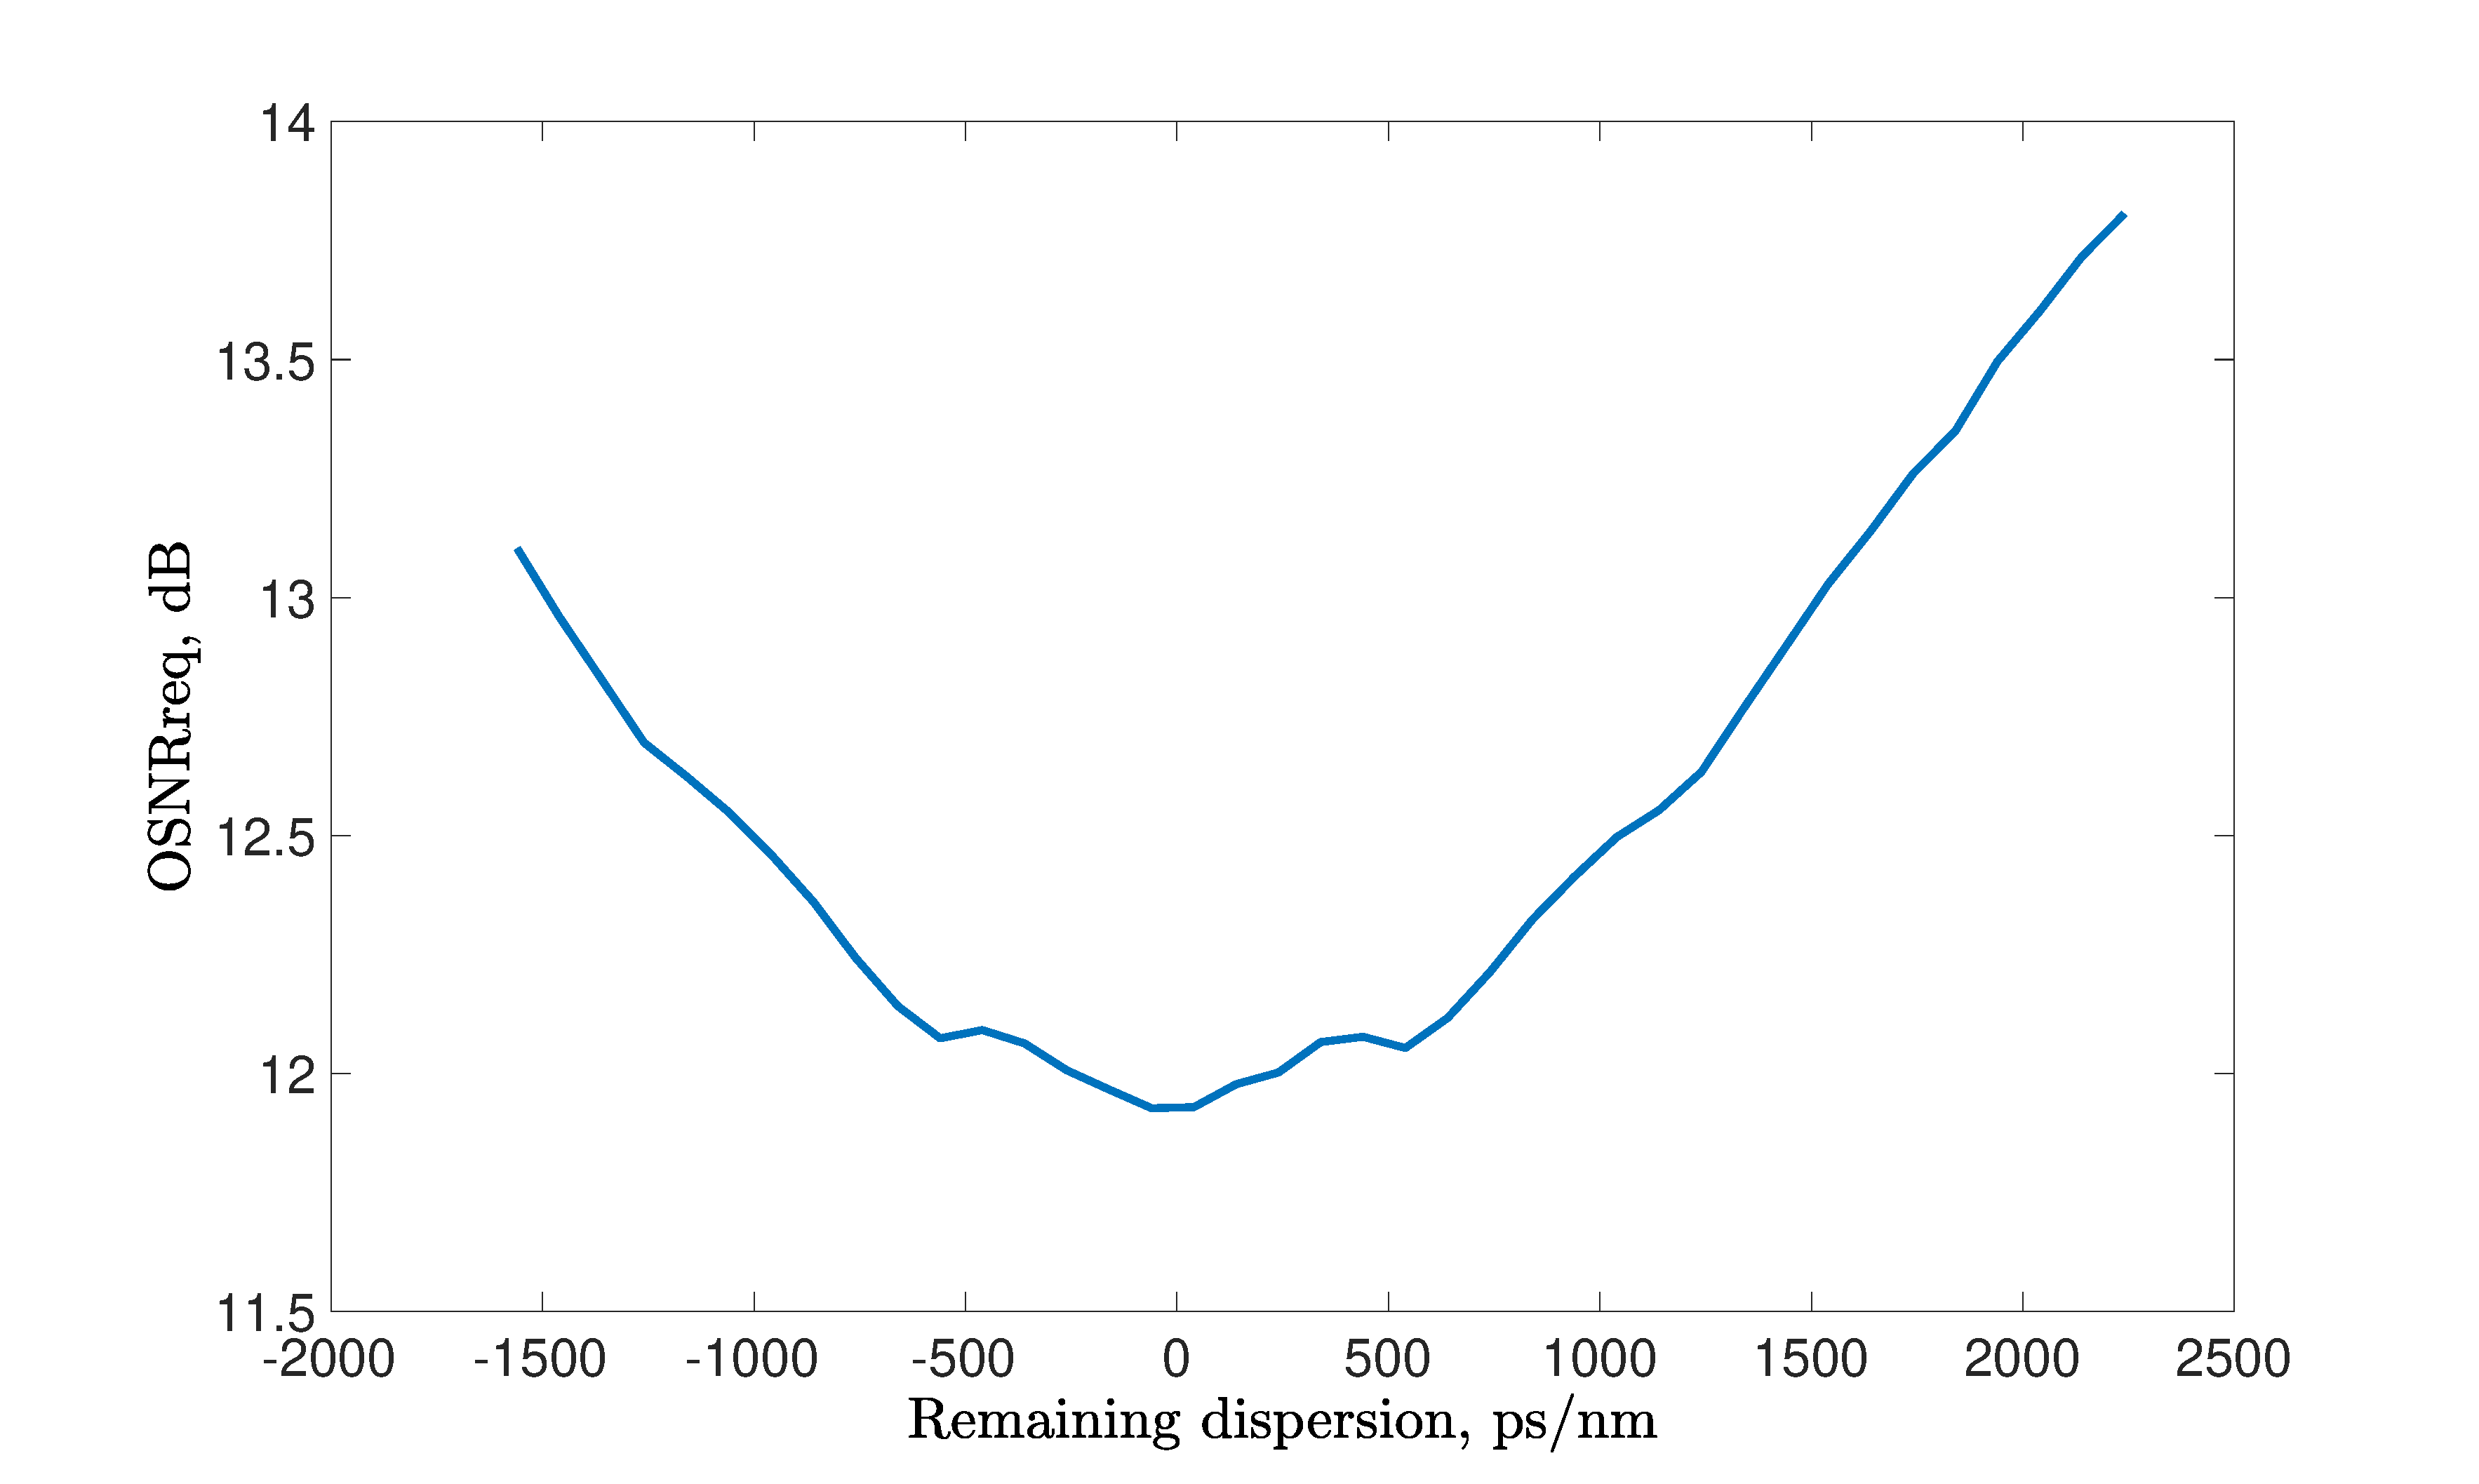
\includegraphics[width=0.8\linewidth]{OSNRreqVsRemDisp.eps}
	\caption{Расчетная кривая требуемого OSNR от остаточной дисперсии}
	\label{fig:ExpSetup}
\end{figure}
\end{document}
